\documentclass[11pt, letterpaper, includehead]{article}

%%%%%%%%%%%%%%%%%%%%% Pre-document %%%%%%%%%%%%%%%%%%%%%
\usepackage{fancyhdr}  % Allow for headers
\usepackage{graphicx}  % Allow for figures 
\usepackage{float}     % Allow for figure inserted in specified location
\usepackage{amsmath}   % Allow for aligned math
\usepackage{array}     % Allow for cell width manipulation
\usepackage{nicematrix}
\usepackage{amssymb} % Uhhhh what was this????
\usepackage{multicol}

\setlength{\parindent}{0pt} % Remove auto paragraph indents

% Get rid of those big ass margins
\usepackage[margin=1in]{geometry}

% Table cell formatting
\setlength{\arrayrulewidth}{0.25mm}
\setlength{\tabcolsep}{11pt}
\renewcommand{\arraystretch}{1.2}

\begin{document}

%%%%%%%%%%%%%%%%%%%%% Title Page %%%%%%%%%%%%%%%%%%%%%
\begin{titlepage}
  \begin{center}
    \Huge{\textbf{Lab 8}}\\
    \Huge{Conservation of Energy}
    \vfill
    \begin{figure}[H] % H makes the figure insert at the position in the document
      \centering 
      \includegraphics[width=6cm]{../logo.png}
    \end{figure}
    \large{\textbf{your name here}}\\
    \large{Julian Barossi, Liam Gilligan, Stephanie L'Heureux}\\
    \vspace{0.5cm}
    \normalsize
    \today
  \end{center}
\end{titlepage}

%%%%%%%%%%%%%%%%%%%%% TABLE OF CONTENTS %%%%%%%%%%%%%%%%%%%%%
\tableofcontents
\pagebreak % Move to next page

% Add a nice fancy header
\pagestyle{fancy}
\fancyhead{}
\fancyhead[C]{\textbf{Lab 8:} Conservation of Energy}

\section{Mass-spring system} % 1
\textbf{Focus on one complete cycle of the mass-spring system and indicate 
on your plot the two turning points (lower and higher) and the equilibrium point.}\\

\begin{multicols}{2}
\begin{figure}[H] % H makes the figure insert at the position in the document
  \centering 
  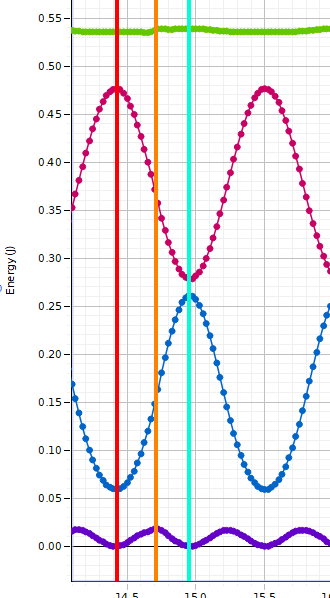
\includegraphics[width=5cm]{graph.png}
\end{figure}
\columnbreak

% Define colors 
\definecolor{purple}{RGB}{93, 63, 211}
\definecolor{green}{RGB}{76, 187, 23}

\begin{center} 
  \begin{tabular}{| m{1cm} |  m{1cm} | m{1cm} |m{1cm} |} 
    \hline
     \boldmath{$U_s$} & \boldmath{$U_g$} & \boldmath{$E_{tot}$} & \boldmath{$K$}\\ 
      \hline
      \Large\textcolor{blue}{\ensuremath\bullet} & \Large\textcolor{magenta}{\ensuremath\bullet} &  \Large\textcolor{green}{\ensuremath\bullet} & \Large\textcolor{purple}{\ensuremath\bullet}\\
      \hline
  \end{tabular} 
\end{center}
\begin{center} 
  \begin{tabular}{| m{2cm} |  m{2.3cm} | m{2.5cm} |} 
    \hline
     \textbf{High Turning Point} & \textbf{Equilibrium} & \textbf{Low Turning Point}\\ 
      \hline
      \Large\textcolor{red}{\ensuremath\bullet} & \Large\textcolor{orange}{\ensuremath\bullet} &  \Large\textcolor{cyan}{\ensuremath\bullet}\\
      \hline
  \end{tabular} 
\end{center}
\end{multicols}

\subsection{High Turning Point}
\textbf{Is $U_g$ is a minimum, a maximum, or neither? Explain why.}\\
At the high turning point, $U_g$ is at a maximum. We can see this in the graph,
and logically the height and therefore gravitational potential energy will be at
a maximum right before it starts moving downwards.\\
\textbf{Is $U_{sp}$ is a minimum, a maximum, or neither? Explain why.}\\
$U_{sp}$ is at a minimum, which we can again see graphically. Logically, the
spring potential will be lowest at the top right before it begins accelerating
downwards, as that is when the spring will have the smallest displacement from 
equilibrium.\\
\textbf{Is $K$ is a minimum, a maximum, or neither? Explain why.}\\
$K$ will be at a minimum at the high turning point, as just a moment before
it will be moving upwards and just a moment after it will be moving
downwards, and is therefore at rest. The graph confirms this logic.

\subsection{Equilibrium}
\textbf{Is $U_g$ is a minimum, a maximum, or neither? Explain why.}\\
$U_g$ is neither at a minimum nor a maximum, as it is at neither the highest
nor lowest points.\\
\textbf{Is $U_{sp}$ is a minimum, a maximum, or neither? Explain why.}\\
Similarly, $U_{sp}$ will neither be at a minimum nor a maximum, as the spring
will be slightly compressed, but not fully.\\
\textbf{Is $K$ is a minimum, a maximum, or neither? Explain why.}\\
$K$ is at a maximum, as we can see that we are at an inflection point in the 
graph of $U_g$. Because $U_g \propto h_{weight}$ and the mass and acceleration
due to gravity is constant, the slope or $\frac{d}{dt}U_g$ will be the velocity
of the weight. Because there is an inflection point in the graph of $U_g$, we 
can see that the velocity is increasing before and then decreasing after, meaning
it is at a maximum. The graph of kinetic energy also shows a maximum at this point.

\subsection{Low Turning Point}
\textbf{Is $U_g$ is a minimum, a maximum, or neither? Explain why.}\\
$U_g$ is at a minimum, as the low turning point will be the lowest point the weight
reaches.
\textbf{Is $U_{sp}$ is a minimum, a maximum, or neither? Explain why.}\\
$U_{sp}$ is at a maximum, as at the lowest point the displacement of the spring will
be at a maximum.
\textbf{Is $K$ is a minimum, a maximum, or neither? Explain why.}\\
$K$ will be at a minimum, as the speed must be zero at the turning points.

\subsection{}
\textbf{Why does the kinetic energy curve peak twice per cycle?}\\
Because on both the way up as well as the way down there will be a point where the
force in the direction of the weight's movement is equal to the force opposing its 
motion, but has been greater at every point since the weight was at rest (e.g.
gravity is greater than spring force from when the weight is at the high turning
point until it reaches equilibrium).\\
\textbf{Is mechanical energy conserved? Justify your answer with 
data. If not, can you identify (and possibly eliminate) systematic 
errors in your data?}\\
The total energy of the system is indicated with a green line on the graph above.
throughout the experiment, the green line remained at around the same value, with 
the systems kinetic, gravitational potential, and spring energy only ever increasing
with a corresponding decrease of one of the other energies. Because of this,
mechanical energy is conserved throughout the experiment.
\section{Conservation of energy}
\subsection{Procedure}
Our experiment used a spring to launch a cart up an inclined ramp. By knowing the spring
constant of the launch spring and compressing the cart a known distance, we can predict the
final height of the cart.
\begin{enumerate} 
  \item Find the Spring Constant $k$ of the spring. To do this, push the cart on the force
  sensor and hold it at a given distance. Read the force that is being applied to the sensor.
  Since the cart is not moving, you know $\sum \vec{F} = 0$, and thereforce $|F_{push}| = |F_{spring}|$.
  Therefore: $|F_{push}| = k\Delta x$ and $k = \frac{|{F}_{push}|}{\Delta x}$.
  \item Measure the angle of the incline by measuring the adjacent and opposite lengths
  then taking the $\arctan$ to find $\theta$.
  \item Position the track at an incline with the spring launcher at the bottom 
        and the motion sensor at the top. 
  \item Use a distance sensor to measure the position of the cart after the launch, the peak it measures
        will be the highest point.
\end{enumerate}

\subsection{Data}
Below is a table of the distance from the launch point (distance while compressed)
for each trial.
\begin{center} 
  \begin{tabular}{|  m{2cm} | m{3cm} |} 
    \hline
    \textbf{Attempt} & \textbf{Distance ($x_f$)} \\ 
    \hline
    1 & 0.190\\ 
    \hline
    2 & 0.179\\ 
    \hline
    3 & 0.171\\ 
    \hline
    4 & 0.181\\ 
    \hline
    5 & 0.179\\ 
    \hline
    6 & 0.177\\ 
    \hline
    7 & 0.168\\ 
    \hline
    8 & 0.177\\ 
    \hline
    9 & 0.165\\ 
    \hline
    10 & 0.176\\ 
    \hline
  \end{tabular} 
\end{center}

\subsection{Data analysis}
\subsubsection{Expected Value}
% Add finding k
Our predicted distance along the track, $x_{thy}$, can be predicted using
the laws of conservation of mechanical energy - and do not regard any nonconservative
forces. In our system, which we define as the cart as well as the Earth, we determine
that initially the system only has potential spring energy ($U_{spring}$), and at the highest
point will only have gravitational potential energy ($U_g$). 


$$U_{spring_i} = U_{g_f}$$
$$\frac{1}{2}k\Delta x^2 = mgh_f$$
$$h_f = \frac{k\Delta x^2}{2mg}$$

There are two important details about this setup which must be noted:\\
\begin{enumerate}
  \item It is assumed that the cart has no gravitational potential energy
        when the spring is compressed, not when the spring is at equilibrium.
        This means the final height will be above where the cart is when it is compressed.
  \item The height given by the final gravitational potential energy is not
        the distance along the track ($h_f \ne x_f$), and is instead the 
        displacement opposite to the direction of gravity. We can find $x_f$ using simple trigonometry
        ($x_f = \frac{h_f}{\sin\theta}$)  
\end{enumerate}

Now to calculate our value for $x_{thy}$, we plug our measured values
into the equations listed above:

\begin{multicols}{2}
  $$k = \frac{|{F}_{push}|}{\Delta x}$$
  $$k = \frac{2.86N}{0.025}$$
  $$k = 114.4N/m$$

  \columnbreak

  $$\tan\theta = \frac{\text{opposite}}{\text{adjacent}}$$
  $$\theta = \arctan\left(\frac{\text{opposite}}{\text{adjacent}}\right)$$
  $$\theta = \arctan\left(\frac{0.90m}{0.155m}\right)$$
  $$\theta = 9.7717^{\circ}$$

\end{multicols}

$$h_f = \frac{k\Delta x^2}{2mg}$$
$$h_f = \frac{114.4N/m\cdot(0.04m)^2}{2\cdot0.2996kg\cdot9.80m/s^2}$$
$$h_f \approx 0.031170m$$\\
$$x_{thy} = \frac{h_f}{\sin\theta}$$
$$x_{thy} = \frac{0.031170m}{\sin9.7717^{\circ}}$$\\
$$x_{thy} = \boxed{0.183657m}$$\\

\subsubsection{Calculating Average, Standard Deviation, and Standard Error}
Below are our values for the mean distance from launch point ($x_f$), as well
as our standard deviation and standard error, calculated using the normal formulas.

\begin{center} 
  \begin{tabular}{|  m{4cm} | m{3cm} | } 
    \hline 
    \textbf{Quantity} & \textbf{Value}\\
    \hline
    Average ($\bar{x}_f$) & 0.176  \\ 
    \hline
    Standard Deviation ($\sigma$)& 0.007\\ 
    \hline
    Standard Error & 0.002\\ 
    \hline      
  \end{tabular} 
\end{center}


\subsubsection{Is the experiment consistent with theory?}
For this experiment to be consistent with theory, our average final distance
$\bar{x}_f$ should be within $\pm 2SE$ from our expected final distance $x_{thy}$.

$$x_{thy} - 2SE \le \bar{x}_f \le x_{thy} + 2SE$$
$$0.183657m - 2\cdot 0.002m \le 0.176m \le 0.183657m + 2\cdot 0.002m$$
$$0.179657m \nleq 0.176m \le 0.187657m$$

From the calculations above, we see that our measured value does not fall between
2 standard errors from the theoretical value.
\subsection{Conclusion}
While our methodology was sound, we did not get accurate enough results to fall within 
2 standard errors. It is likely for a combination of two factors:
\begin{enumerate}
  \item We were too precise in our measurements. We made sure to line up the cart to the exact same
        location everytime, and used a small $\Delta x$, as $\Delta x$ gets bigger any small inaccuracies
        will result in a greately different initial energy ($U_{spring} \propto \Delta x^2$).
  \item We did not account for friction or drag. These nonconservative forces will result
        in the cart not reaching as high of a final height as we were expecting, as energy 
        that would normally be converted into gravitational potential energy is instead converted
        into heat.
\end{enumerate}
Because of factor 1, our standard deviation was very low, and therefore our standard error was very low. Because
of factor 2, the $x_f$ we will measure will be lower than $x_{thy}$, and because our standard error is so low it
would have to be very close to fall within that range.

\end{document}